%For arXiv main file is the one that has document class
\documentclass[a4paper,fleqn]{latex_styles/cas-sc}
%% 
%% Copyright 2019-2020 Elsevier Ltd
%% 
%% This file is part of the 'CAS Bundle'.
%% --------------------------------------
%% 
%% It may be distributed under the conditions of the LaTeX Project Public
%% License, either version 1.2 of this license or (at your option) any
%% later version.  The latest version of this license is in
%%    http://www.latex-project.org/lppl.txt
%% and version 1.2 or later is part of all distributions of LaTeX
%% version 1999/12/01 or later.
%% 
%% The list of all files belonging to the 'CAS Bundle' is
%% given in the file `manifest.txt'.
%% 
%% Template article for cas-sc documentclass for 
%% double column output.

%\documentclass[a4paper,fleqn,longmktitle]{cas-sc}
\documentclass[a4paper,fleqn]{latex_styles/cas-sc}

% \usepackage[numbers]{natbib}
%\usepackage[authoryear]{natbib}
\usepackage[authoryear,longnamesfirst]{natbib}


\usepackage{subfigure}
\usepackage{letltxmacro}
\usepackage{hyperref}
\usepackage{amsmath}
\usepackage{booktabs}
\usepackage{longtable}
\usepackage{array}
\usepackage{multirow}
\usepackage{wrapfig}
\usepackage{colortbl}
\usepackage{pdflscape}
\usepackage{tabu}
\usepackage[normalem]{ulem}
\usepackage{makecell}
\usepackage{xcolor}
\usepackage{caption}
\usepackage{tabularx}
\usepackage{adjustbox}
\usepackage{natbib}
\usepackage{mfirstuc}
\usepackage{float}
\usepackage{placeins}
\usepackage{footnote}
\bibpunct{(}{)}{,}{a}{}{;}


\renewcommand{\figurename}{\textbf{Fig.}}

\DeclareCaptionFormat{bold}{\textbf{#1#2}#3}
\captionsetup[table]{format=bold, labelsep=none, justification=raggedright, singlelinecheck=false}
\captionsetup[figure]{format=bold, labelsep=period, singlelinecheck=false}


\setcitestyle{aysep={}}
\setcitestyle{authoryear,open={(},close={)}}



%%%Author definitions
\def\tsc#1{\csdef{#1}{\textsc{\lowercase{#1}}\xspace}}
\tsc{WGM}
\tsc{QE}
\tsc{EP}
\tsc{PMS}
\tsc{BEC}
\tsc{DE}
%%%

% Uncomment and use as if needed
%\newtheorem{theorem}{Theorem}
%\newtheorem{lemma}[theorem]{Lemma}
%\newdefinition{rmk}{Remark}
%\newproof{pf}{Proof}
%\newproof{pot}{Proof of Theorem \ref{thm}}



\begin{document}
\let\WriteBookmarks\relax
\def\floatpagepagefraction{1}
\def\textpagefraction{.001}

% Short title
\shorttitle{Sources of capital growth}

% Short author
\shortauthors{Gordon Getty}

% Main title of the paper
\title [mode = title]{Sources of capital growth}                      
% Title footnote mark
% eg: \tnotemark[1]
% \tnotemark[1,2]
% Title footnote 1.
% eg: \tnotetext[1]{Title footnote text}
% \tnotetext[<tnote number>]{<tnote text>} 
% \tnotetext[1]{This document is the results of the research
%   project funded by the National Science Foundation.}

% \tnotetext[2]{The second title footnote which is a longer text matter
%   to fill through the whole text width and overflow into
%   another line in the footnotes area of the first page.}


% First author
%
% Options: Use if required
% eg: \author[1,3]{Author Name}[type=editor,
%       style=chinese,
%       auid=000,
%       bioid=1,
%       prefix=Sir,
%       orcid=0000-0000-0000-0000,
%       facebook=<facebook id>,
%       twitter=<twitter id>,
%       linkedin=<linkedin id>,
%       gplus=<gplus id>]
\author[1]{Gordon Getty}[
                        type=editor,
                       % auid=000,bioid=1,
                       % prefix=Sir,
                        role=Researcher,
                        orcid=0000-0002-0939-6932
                        ]

\ead{ggetty@LeakeyFoundation.org}

\author[2]{Nikita Tkachenko}[
                        type=editor,
                       % auid=000,bioid=1,
                       % prefix=Sir,
                        role=Assistant,
                        orcid=0009-0003-8681-3335
                        ]

% Corresponding author indication
\cormark[1]

\ead{natkachenko@usfca.edu}
% Footnote of the first author
% \fnmark[1]

% Email id of the first author

% URL of the first author
% \ead[url]{www.cvr.cc, cvr@sayahna.org}

%  Credit authorship
% \credit{Conceptualization of this study, Methodology, Software}

% Address/affiliation
\affiliation[1]{organization={Fellow, UCB},
            addressline={University Avenue and, Oxford St}, 
            city={Berkeley},
            postcode={94720}, 
            state={California},
            country={United States}}
            
\affiliation[2]{organization={Graduate Student, University of San Francisco},
            addressline={2130 Fulton St}, 
            city={San Francisco},
            postcode={94117}, 
            state={California},
            country={United States}}

% Second author
% \author[2,4]{Han Theh Thanh}[style=chinese]

% Third author
%\author[2,3]{CV Rajagopal}[%
%   role=Co-ordinator,
%   suffix=Jr,
%   ]
%\fnmark[2]
%\ead{cvr3@sayahna.org}
%\ead[URL]{www.sayahna.org}

%\credit{Data curation, Writing - Original draft preparation}

% Address/affiliation
% \affiliation[2]{organization={Sayahna Foundation},
%    % addressline={}, 
%    city={Jagathy},
%    % citysep={}, % Uncomment if no comma needed between city and postcode
%    postcode={695014}, 
%    state={Trivandrum},
%    country={India}}

% Corresponding author text
\cortext[cor1]{Corresponding author}
% \cortext[cor2]{Principal corresponding author}

% Footnote text
%\fntext[fn1]{This is the first author footnote. but is common to third
%  author as well.}
%\fntext[fn2]{Another author footnote, this is a very long footnote and
%  it should be a really long footnote. But this footnote is not yet
%  sufficiently long enough to make two lines of footnote text.}

% For a title note without a number/mark
%\nonumnote{This note has no numbers. In this work we demonstrate $a_b$
%  the formation Y\_1 of a new type of polariton on the interface
%  between a cuprous oxide slab and a polystyrene micro-sphere placed
%  on the slab.
%  }

% Here goes the abstract
\begin{abstract}
Data from national accounts show no effect of change in net saving,
in ratio to market-value capital, on change in growth
rate of market-value capital (capital acceleration). Thus it appears
that capital growth and acceleration arrive without help from net
saving. We explore ways in which this is
possible, and discuss implications for economic teaching and public
policy.     
\\ % So keywords fit
\end{abstract}

% Use if graphical abstract is present
% \begin{graphicalabstract}
% \includegraphics{figs/grabs.pdf}
% \end{graphicalabstract}

% Research highlights
%\begin{highlights}
%\item Research highlights item 1
%\item Research highlights item 2
%\item Research highlights item 3
%\end{highlights}

% Keywords
% Each keyword is seperated by \sep
\begin{keywords}
National accounts \sep Net
saving \sep Market-value capital \sep Capital
growth \sep 
Capital acceleration

\end{keywords}

\maketitle

\hypertarget{introduction}{%
\section{Introduction and overview}\label{introduction}}

Many economists over the centuries have reasoned that net saving, or equivalently net investment\footnote{As reported in national accounts; they differ only by statistical discrepancy. Also see Appendix \hyperref[appendix-a]{A}.}, should tend to give equal capital growth. Economists since the early
nineteenth century have added the proviso that net saving cannot
safely outpace innovation; more capital must mean capital redesigned for
greater productivity if economies are to escape risk of capital glut and
diminishing returns
(\citet{westEssayApplicationCapital1815, ricardoEssayProfitsVol1815, malthusEnquiryNatureProgress1815}).
Roy \citet{harrodEssayDynamicTheory1939}
described that limit for safe net saving, meaning the rate of
imagining and developing new ideas for more productive forms of capital,
as the ``warranted rate''. Harrod, and many other economists of his time
and since, have focused on growth of output rather than of capital, but
have modeled growth of output by first assuming the equivalence of net
saving and capital growth, within the warranted rate, and then
looking for effects of that capital growth on later output growth.

Some other economists, including John  \citet{raeNewPrinciplesPolitical1834} and John Stuart 
\citet{millPrinciplesPoliticalEconomy1848} (see Appendix \hyperref[appendix-c]{C}), argued that capital growth might also be explained
by a rise in productivity of capital and labor already extant. Ways
might be found for existing factors to produce more, that is, and so to
allow more consumption, or more capital growth, or any mix of the two,
without inputs of net saving. Robert
\citet{solowTECHNICALCHANGEAGGREGATE1957} allowed that possibility for
``disembodied'' growth, where plant and products already existing are
repurposed or redeployed in more productive ways.

We test between those two explanations of capital growth, by net
saving or by increase in productivity of capital and labor already
in existence, by comparing net saving to concurrent change in
market-value capital in 92 countries. All data are drawn from national accounts
of those countries as collated on the free website \href{https://wid.world/}{World Inequality Database}.

Those test results from data for net saving/capital ratio 
are easiest to reconcile in an interpretation that net saving has no effect on capital growth.
Net saving, if so, raises the physical quantity of capital, but not the
aggregate value, and so reduces the value per unit.

The data are most easily explained by the present value principle,
and by production efficiencies enabled through innovation. Value is
created in the mind of the market at the moment when prospective cash
flows are discounted. It is created only if the market sees a path, step
by step, from the start, to practical realization of those prospective
cash flows. Then capital growth arrives when the market first evaluates
prospective cash flows, and is realized eventually in physical outcomes
insofar as the market has predicted correctly. That is to say that capital
growth, in the mind of the market, precedes and pays for any needed investment
in new plant and equipment.\footnote{Present value is time-discounted, and affords innovators only enough, at first, for first steps in implementation. As implementation proceeds, present value rises and affords more.}

Meanwhile the innovator
acquires materials and plant capacity and labor skills at market prices
determined by their uses in current technology, but applies them more
productively until competition catches up. It is that temporary market
advantage to the innovator which explains capital growth without net
saving in a practical and mechanical sense, while the present value
principle gives the explanation in terms of market valuation. This idea
will be called ``free growth theory'' for easy reference.

It predicts only at the largest scales, and only for the private sector.
Individuals and groups and even small economies can grow
or decline through net saving or dissaving. That possibility is foreclosed only at the
scale of all capital and all economies together. The public sector,
meanwhile, responds to political rather than market choices, and grows
or shrinks accordingly.

If free growth theory is right, tax policy and other policy to encourage
saving over consumption should be reviewed. These policies
include the higher tax on ordinary income than on capital gains, and the
double tax on corporate dividends.

Inferences for economic teaching include the obvious ones for growth
theory and for net saving in general. They include others as well.
One of the central doctrines of the marginalist revolution has held that
market realization converges to producer cost, when that cost includes
imputed interest on assets owned. Net saving gives producer cost,
and falls short of market realization in the presence of technological
growth from new ideas. Meanwhile the doctrine that net income equals
consumption plus net saving is put into question by evidence offered
here suggesting that net saving increases the physical quantity of
capital, but not the aggregate value. In general, economics might
consider relying less on book value and net investment, and more on market value and on the
power of ideas.

\hypertarget{net-saving-and-capital-growth}{%
\section{Net saving, capital growth and capital acceleration}\label{net-saving-and-capital-growth}}

Thrift theory will mean the combined ideas that all net saving \(S_{net}\) is realized in equal growth of capital \(K\), if \(S_{net}\) holds within the warranted rate, and that there is no other source of capital growth except market noise regressing to zero. "Thrift assumptions" will mean those two plus the assumptions that current \(S_{net}\) holds within the warranted rate. The acronym uta will mean "under thrift assumptions." Then 
%
\begin{equation}
    \Delta K = S_{net}\ ,\quad \text{uta}. \label{eq-1}
\end{equation}
%
Define "thrift" \(s^*\) by \(s^* = \frac{S_{net}}{K}\), and divide Eq. \eqref{eq-1} by capital to predict capital growth rate \(g(K)\) as
%
\begin{equation}
g(K) = s^* \ , \quad \text{uta,}\quad \text{where } s^* = \frac{S_{net}}{K}.\quad \text{ Then} \label{eq-2}
\end{equation}
%
\vspace{-5ex}
%
\begin{equation}
\Delta g(K) = \Delta s^*\ , \quad \text{uta.} \label{eq-3}
\end{equation}
%
\(\Delta g(K)\) and \(\Delta s^*\) respectively will be called "capital acceleration" and "thrift change," either of which may be positive or negative. Division of Eq. \eqref{eq-3} by capital acceleration, with rearrangement, gives
%
\begin{equation}
\frac{\Delta s^*}{\Delta g(K)} = \frac{\Delta g(K)}{\Delta g(K)} = 1\ , \quad \text{uta}. \label{eq-4}
\end{equation}
%

The argument has continued from growth in Eq. \eqref{eq-2} to acceleration in Eqs. \eqref{eq-3} and \eqref{eq-4} on the reasoning that causal relationships among variables, in this case between thrift and capital growth rate, tend to be revealed most reliably in their concurrent changes. Eq. \eqref{eq-4} was derived from Eq. \eqref{eq-3} so that success of predictions from growth assumptions can be measured against a standard of unity. For notational convenience, then, we define the "thrift index" \(\theta\) by \(\theta = \frac{\Delta s^*}{\Delta g(K)}\), and restate Eq. \eqref{eq-4} as
%
\begin{equation}
\theta = 1\ , \quad \text{uta,}\quad \text{where} \ \theta = \frac{\Delta s^*}{\Delta g(K)}\ . \label{eq-5}
\end{equation}
%

Test results for the predictions \(\frac{s^*}{g(K)} = \frac{\Delta s^*}{\Delta g(K)} = 1\), under thrift assumptions, appear in Fig. \ref{fig-s_c_theta_plots} and in Tables \ref{tbl-reg_s}, \ref{tbl-5} and \ref{tbl-indicator_table}. Results were found as GDP-weighted averages over all countries and years, from data for net saving and market-value capital taken from national accounts. They show \(\frac{s^*}{g(K)} = 0.481\), with regression of \(s^*\) on \(g(K)\) found at 0.0771, and \(\frac{\Delta s^*}{\Delta g(K)} = 0.064\), with regression of \(\Delta s^*\) on \(\Delta g(K)\) at 0.0559.

\FloatBarrier
\begin{figure}[pos=H]
    \centering
    % \subfigure{
        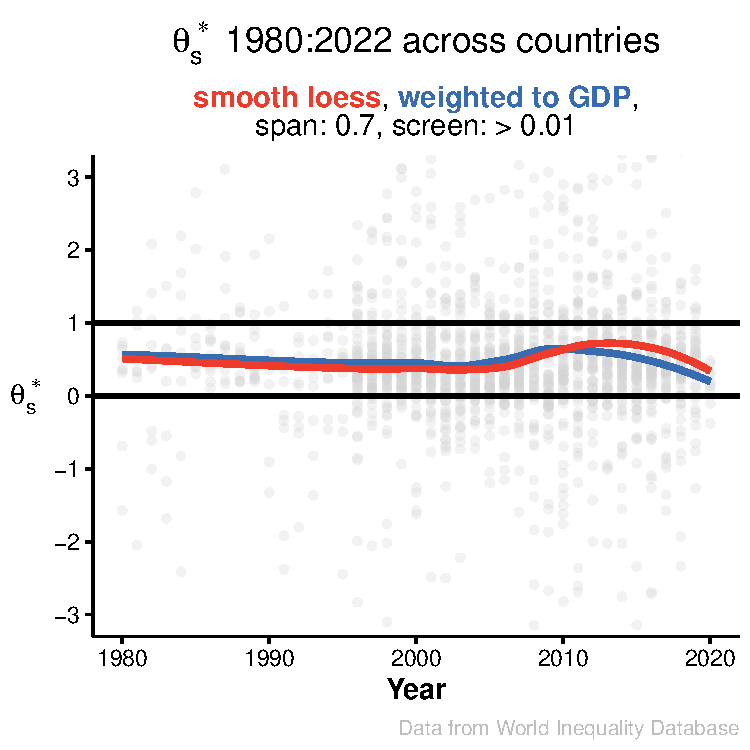
\includegraphics[width=1\textwidth]{./figure-pdf/fig-s_c_theta_plots-1.pdf}
        % \label{fig-s_c_theta_plots-1-new}
    % }
    % \quad % This adds some space between the two subfigures
    % \subfigure{
    %     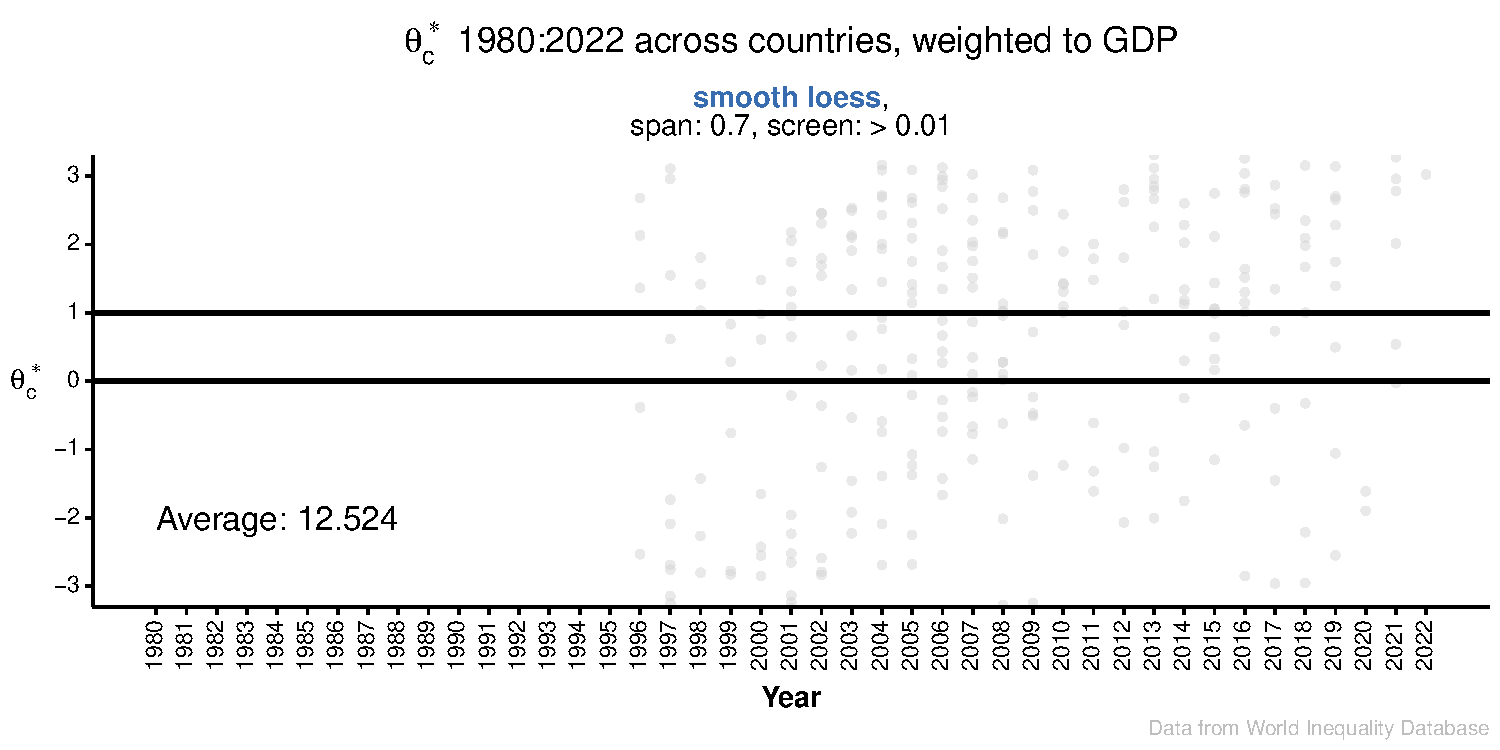
\includegraphics[width=0.45\textwidth]{./figure-pdf/fig-s_c_theta_plots-2.pdf}
    %     \label{fig-s_c_theta_plots-2}
    % }
    \captionsetup{justification=centering}
    \caption{\textcolor[HTML]{EF3B2C}{Average \(\frac{s^*}{g(K)}\)} with \textcolor[HTML]{386CB0}{LOESS smoothing} over all countries, GDP-weighted, 1980-2022} % and \(\theta^*_c\)
    \label{fig-s_c_theta_plots}
\end{figure}
%
\vfill
%
% \begin{table}[pos=h]
\caption{Regression of \(s^*\) on \(g(K)\) and \(\Delta s^*\) on \(\Delta g(K)\), GDP-weighted. Screen = 0.01. \(H_0\) per thrift theory: \(\frac{s^*}{g(K)} = \frac{\Delta s^*}{\Delta g(K)} = 1\).}
\centering
\begin{tabularx}{\columnwidth}{lcc}
   \toprule
                                               & $s^*$          & $\Delta s^*$ \\    
   \midrule 
   Regression of $s^*$ on \(g(K)\)             & 0.0771$^{***}$ &   \\   
                                               & (0.0144)       &   \\   
   Regression of value shown on $\Delta g(K)$  &                & 0.0559$^{***}$\\   
                                               &                & (0.0057)\\   
    \\
   Observations                                & 1,826          & 1,574\\  
   R$^2$                                       & 0.84511        & 0.37071\\  
   Within R$^2$                                & 0.10669        & 0.27233\\  
    \\
   Year fixed effects                          & $\checkmark$   & $\checkmark$\\   
   Country fixed effects                       & $\checkmark$   & $\checkmark$\\   
   \bottomrule
\end{tabularx}
   \label{tbl-reg_s}
\end{table} % Table 4
\begin{table}[pos=h]
    \caption{Regression of \(s^*\) on \(g(K)\) and \(\Delta s^*\) on \(\Delta g(K)\), GDP-weighted. Screen = 0.01. \(H_0\) per thrift theory: \(\frac{s^*}{g(K)} = \frac{\Delta s^*}{\Delta g(K)} = 1\).\label{tbl-reg_s}}
    \hrule
    \centering
\begin{minipage}{0.45\textwidth}
\begin{table}[pos=h]
\caption{Regression of \(s^*\) on \(g(K)\), GDP-weighted (Screen = 0.01). \(H_0\) per thrift theory: \(g(K) = s^*\) \& \(\frac{s^*}{g(K)} = 1\).}
\centering
\begin{tabularx}{\columnwidth}{lcc}
   \toprule
                                     & $s^*$ \\   
   \midrule 
   Regression of $s^*$ on \(g(K)\)   & 0.0771$^{***}$\\   
                                     & (0.0144)\\   
    \\
   Observations                      & 1,826\\  
   R$^2$                             & 0.84511\\  
   Within R$^2$                      & 0.10669\\  
    \\
   Year fixed effects                & $\checkmark$\\   
   Country fixed effects             & $\checkmark$\\   
   \bottomrule
\end{tabularx}
   \label{tbl-4}
\end{table}
\end{minipage}
\hfill
    \begin{minipage}{0.45\textwidth}
\begin{table}[pos=h]
\caption{Regression of $\Delta s^*$ and $\Delta q_s$ on $\Delta g(K)$ (Screen = 0.01). $H_0\ \text{per thrift theory:} \ \Delta g(K) \cong \Delta s^* \ \& \ \Delta q_s \cong 0$}
\centering
\begin{tabularx}{\columnwidth}{lcc}
   \toprule
                                               & $\Delta s^*$   & $\Delta q_s$ \\    
   \midrule 
   Regression of value shown on $\Delta g(K)$  & 0.1092$^{***}$ & 0.8908$^{***}$\\   
                                               & (0.0163)       & (0.0163)\\   
    \\
   Observations                                & 1,412          & 1,412\\  
   R$^2$                                       & 0.32023        & 0.95280\\  
   Within R$^2$                                & 0.22472        & 0.95076\\  
    \\
   year fixed effects                          & $\checkmark$   & $\checkmark$\\   
   country fixed effects                       & $\checkmark$   & $\checkmark$\\   
   \bottomrule
\end{tabularx}
   \label{tbl-wid_si_table}
\end{table}
\end{minipage}
\hrule
\end{table}
%
\vfill
%
\begin{figure}[pos=H]
    \centering
    % \subfigure{
        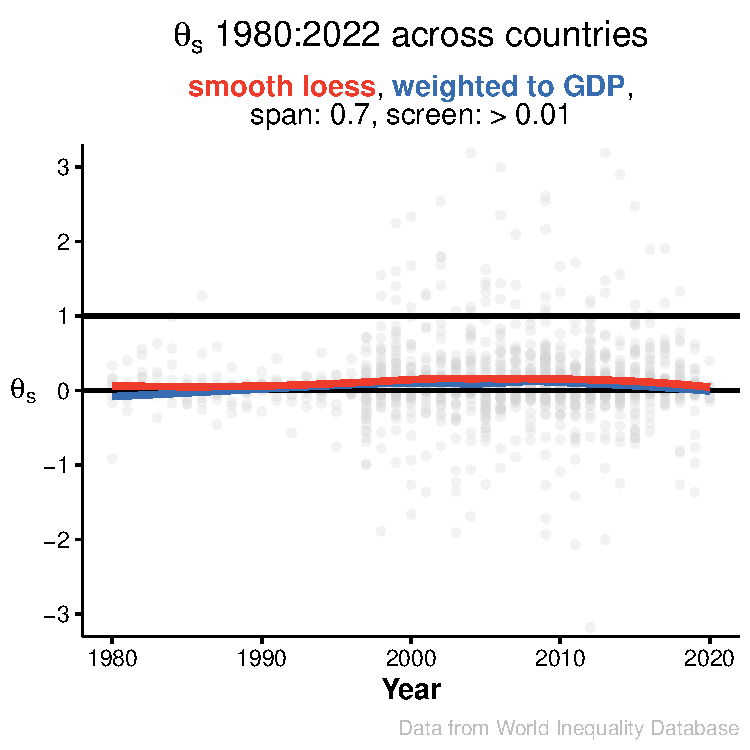
\includegraphics[width=1\textwidth]{./figure-pdf/fig-si_plots-1.pdf}
    %     \label{fig-si_plots-1}
    % }
    % \quad % This adds some space between the two subfigures
    % \subfigure{
    %     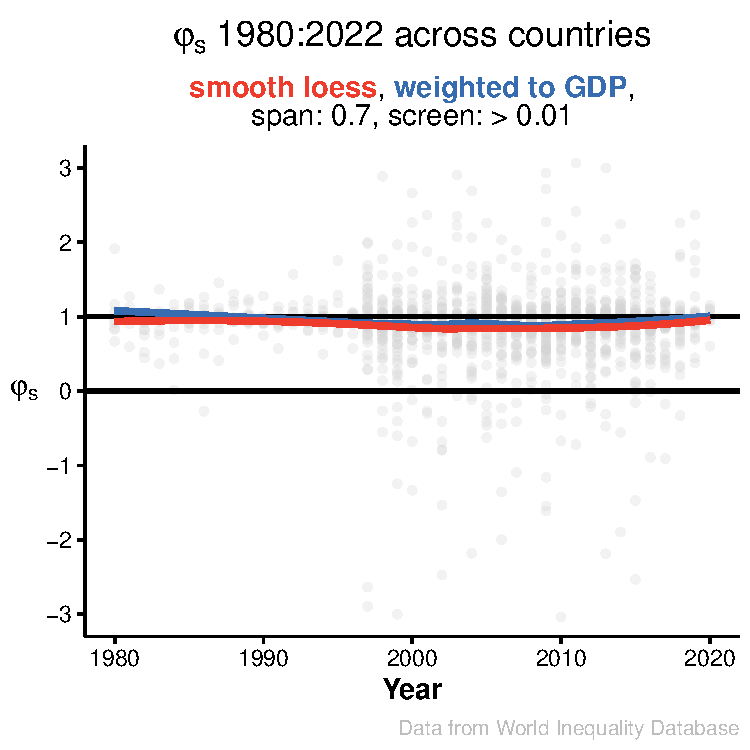
\includegraphics[width=0.45\textwidth]{./figure-pdf/fig-si_plots-2.pdf}
    %     \label{fig-si_plots-2}
    % }
    \captionsetup{justification=centering}
    \caption{\textcolor[HTML]{EF3B2C}{Average \(\theta_s^*\)} with \textcolor[HTML]{386CB0}{LOESS smoothing} over all countries, GDP-weighted, 1980-2022} % and \(\theta^*_c\)
    \label{fig-si_plots}
\end{figure}
%
\FloatBarrier
\begin{table}[pos=h]
\caption{Average \(\frac{s^*}{g(K)}\) in 92 countries (screen = 0.01). Number of years clearing screen shown in ()}\label{tbl-5}%
\toprule
\makebox[\textwidth][c]{%
{\centering

\begin{tabular}{llrr} Armenia & 1996 - 2020 (23) & -0.63\\
Aruba & 1996 - 2001 (6) & 1.25\\
Australia & 1980 - 2018 (33) & 0.24\\
Austria & 1996 - 2021 (23) & 0.83\\
Azerbaijan & 1996 - 2020 (23) & 1.57\\
\addlinespace
Bahrain & 2009 - 2013 (5) & -2.43\\
Belgium & 1996 - 2021 (21) & 0.61\\
Bolivia & 1998 - 2015 (17) & 0.40\\
Botswana & 1996 - 1999 (4) & 3.54\\
Brazil & 1996 - 2019 (21) & 0.25\\
\addlinespace
British Virgin Islands & 1996 - 1999 (4) & 2.45\\
Bulgaria & 1996 - 2016 (16) & 0.14\\
Burkina Faso & 2000 - 2019 (20) & 0.23\\
Cameroon & 1996 - 2019 (24) & 1.10\\
Canada & 1980 - 2022 (38) & 0.37\\
\addlinespace
Cape Verde & 2008 - 2017 (9) & 0.53\\
Chile & 1997 - 2021 (19) & 0.84\\
China & 1992 - 2020 (29) & 0.81\\
Colombia & 1996 - 2022 (27) & 0.60\\
Costa Rica & 2013 - 2020 (6) & 0.21\\
\addlinespace
Croatia & 1996 - 2021 (24) & 0.43\\
Curaçao & 2001 - 2016 (14) & 1.26\\
Cyprus & 1996 - 2021 (25) & 0.07\\
Czechia & 1994 - 2020 (20) & 0.17\\
Côte d’Ivoire & 1996 - 2000 (5) & 0.29\\
\addlinespace
Denmark & 1996 - 2022 (26) & 0.22\\
Dominican Republic & 1996 - 2016 (10) & 1.52\\
Ecuador & 2008 - 2020 (13) & 0.53\\
Egypt & 1997 - 2015 (19) & 0.92\\
El Salvador & 2015 - 2019 (5) & -0.62\\
\addlinespace
Estonia & 1996 - 2021 (24) & 0.45\\
Finland & 1996 - 2021 (23) & 0.17\\
France & 1980 - 2021 (35) & 0.26\\
Germany & 1980 - 2022 (38) & 0.70\\
Greece & 1996 - 2021 (26) & 0.17\\
\addlinespace
Guatemala & 2002 - 2021 (20) & -0.72\\
Guinea & 2004 - 2010 (5) & 0.72\\
Honduras & 2001 - 2015 (14) & -0.57\\
Hong Kong & 1997 - 2011 (15) & 0.90\\
Hungary & 1996 - 2021 (21) & 0.14\\
\addlinespace
Iceland & 2001 - 2014 (14) & 0.22\\
India & 1999 - 2019 (21) & 0.57\\
Indonesia & 2017 - 2019 (3) & 0.94\\
Iran & 1997 - 2017 (20) & 4.96\\
Ireland & 1996 - 2021 (22) & 0.26\\
\addlinespace
Israel & 1996 - 2019 (24) & 0.46\\ \end{tabular}
}

{\centering
\begin{tabular}{llrr} Italy & 1980 - 2022 (36) & 0.13\\
Japan & 1980 - 2021 (29) & 0.19\\
Kazakhstan & 1997 - 2022 (25) & 0.60\\
Kuwait & 2003 - 2017 (14) & 1.11\\
Kyrgyzstan & 1996 - 2021 (24) & 0.46\\
\addlinespace
Latvia & 1996 - 2021 (24) & -0.23\\
Lithuania & 1996 - 2021 (24) & 0.13\\
Luxembourg & 1996 - 2021 (22) & 0.03\\
Malaysia & 2007 - 2015 (9) & 2.52\\
Malta & 1996 - 2021 (23) & 0.16\\
\addlinespace
Mauritius & 2014 - 2018 (5) & 0.04\\
Mexico & 1996 - 2021 (22) & 0.15\\
Moldova & 1996 - 2019 (22) & -0.91\\
Mongolia & 2006 - 2020 (15) & 0.10\\
Morocco & 1999 - 2021 (23) & 1.13\\
\addlinespace
Netherlands & 1996 - 2021 (23) & 0.51\\
New Zealand & 1996 - 2019 (21) & 0.78\\
Nicaragua & 2007 - 2018 (12) & 0.08\\
Niger & 1996 - 2019 (24) & 0.90\\
Norway & 1981 - 2021 (38) & 0.95\\
\addlinespace
Peru & 2008 - 2021 (14) & 0.76\\
Philippines & 1996 - 2022 (27) & 1.76\\
Poland & 1996 - 2021 (25) & 0.71\\
Portugal & 1996 - 2022 (24) & 0.00\\
Qatar & 2002 - 2017 (14) & 1.89\\
\addlinespace
Romania & 1996 - 2020 (22) & 0.03\\
Russia & 1996 - 2017 (13) & -0.19\\
Saudi Arabia & 2003 - 2009 (7) & 2.65\\
Senegal & 2015 - 2021 (7) & 0.24\\
Serbia & 1998 - 2021 (23) & 0.61\\
\addlinespace
Slovakia & 1996 - 2022 (24) & 0.15\\
Slovenia & 1996 - 2021 (20) & 0.28\\
South Africa & 1996 - 2022 (24) & 0.28\\
South Korea & 1996 - 2020 (24) & 0.63\\
Spain & 1995 - 2021 (25) & 0.32\\
\addlinespace
Sweden & 1980 - 2021 (37) & 0.41\\
Switzerland & 1993 - 2021 (25) & 0.69\\
Tunisia & 1996 - 2011 (16) & 0.29\\
Turkey & 2010 - 2017 (8) & 1.32\\
USA & 1980 - 2021 (38) & 0.31\\
\addlinespace
Ukraine & 1996 - 2019 (21) & 0.17\\
United Kingdom & 1981 - 2021 (36) & 0.16\\
Uruguay & 2016 - 2017 (2) & 1.16\\
Uzbekistan & 2011 - 2021 (10) & 0.21\\
Vanuatu & 2002 - 2007 (6) & 0.29\\
\addlinespace
Venezuela & 1998 - 2019 (20) & 0.55\\ \end{tabular}

}
}
\bottomrule
\begin{flushleft}
\footnotesize \emph{Note:} Thrift theory predicts \(\frac{s^*}{g(K)} = 1\). Free growth theory makes no prediction for these data.
\end{flushleft}
\end{table}
\FloatBarrier
%

\FloatBarrier
\begin{table}[H]
\caption{Average \(\varphi_{s,i}\) and \(\varphi_{c,i}\) in 86 countries (screen = 0.01). Number of years clearing screen shown in ()}%
\makebox[\textwidth][c]{%
{\centering

\begin{tabular}{llrr}
\toprule
Country & Period & $\overline{\varphi_{s,i}}$ & $\overline{\varphi_{c,i}}$\\
\midrule
Armenia & 1997 - 2018 (17) & 0.94 & 1.30\\
Aruba & 1997 - 2001 (5) & -0.38 & 8.98\\
Australia & 1962 - 2019 (41) & 0.97 & 1.09\\
Austria & 1997 - 2013 (11) & 0.93 & 1.11\\
Azerbaijan & 1997 - 2018 (22) & 0.39 & 1.85\\
\addlinespace
Bahrain & 2010 - 2013 (4) & 0.59 & 1.32\\
Belgium & 1997 - 2014 (11) & 0.90 & 1.06\\
Bolivia & 1999 - 2013 (12) & 1.03 & 1.28\\
Botswana & 1997 - 2000 (4) & 0.73 & 1.27\\
Brazil & 1998 - 2018 (20) & 0.86 & 1.21\\
\addlinespace
British Virgin Islands & 1997 - 1999 (3) & 0.35 & 3.63\\
Bulgaria & 1997 - 2017 (15) & 0.99 & 1.21\\
Burkina Faso & 2001 - 2018 (15) & 0.94 & 1.23\\
Cameroon & 1998 - 2003 (6) & 0.35 & 4.59\\
Canada & 1974 - 2020 (37) & 0.91 & 1.11\\
\addlinespace
Cape Verde & 2009 - 2017 (9) & 0.56 & 2.01\\
Chile & 1998 - 2018 (18) & 0.93 & 1.37\\
China & 1993 - 2014 (19) & 0.91 & 1.04\\
Colombia & 1997 - 2019 (17) & 0.98 & 2.26\\
Costa Rica & 2014 - 2017 (4) & 0.97 & 1.09\\
\addlinespace
Croatia & 1997 - 2018 (21) & 0.83 & 2.09\\
Curaçao & 2002 - 2016 (12) & 1.13 & 1.18\\
Cyprus & 1997 - 2018 (19) & 0.94 & 1.11\\
Czechia & 1995 - 2018 (14) & 0.99 & 1.04\\
Côte d’Ivoire & 1997 - 2000 (4) & 1.03 & 1.10\\
\addlinespace
Denmark & 1999 - 2020 (20) & 0.92 & 1.00\\
Dominican Republic & 2007 - 2015 (8) & 0.76 & 1.33\\
Ecuador & 2009 - 2018 (10) & 0.85 & 1.87\\
Egypt & 1998 - 2015 (17) & 1.04 & 1.75\\
Estonia & 1997 - 2017 (15) & 0.93 & 1.11\\
\addlinespace
Finland & 1997 - 2020 (19) & 0.97 & 1.11\\
France & 1952 - 2019 (41) & 0.87 & 1.13\\
Germany & 1971 - 2013 (22) & 1.01 & 1.21\\
Greece & 1997 - 2019 (21) & 0.90 & 1.27\\
Guatemala & 2007 - 2019 (9) & 0.96 & 0.93\\
\addlinespace
Guinea & 2005 - 2010 (6) & 0.94 & 1.27\\
Honduras & 2002 - 2015 (14) & 0.70 & 1.56\\
Hong Kong & 1997 - 2020 (21) & 0.91 & 1.12\\
Hungary & 1997 - 2018 (17) & 0.93 & 1.11\\
Iceland & 2002 - 2014 (13) & 0.85 & 1.07\\
\addlinespace
India & 2000 - 2017 (15) & 0.88 & 1.08\\
Iran & 1998 - 2018 (19) & 0.15 & 1.09\\
Ireland & 1997 - 2019 (20) & 0.96 & 0.96\\
\bottomrule
\end{tabular}
}

{\centering
\begin{tabular}{llrr}
\toprule
Country & Period & $\overline{\varphi_{s,i}}$ & $\overline{\varphi_{c,i}}$\\
\midrule
Israel & 1997 - 2017 (18) & 0.95 & 1.68\\
Italy & 1982 - 2017 (21) & 1.01 & 0.98\\
Japan & 1981 - 2017 (28) & 0.95 & 1.13\\
Kazakhstan & 1997 - 2018 (18) & 0.90 & 1.09\\
Kuwait & 2005 - 2017 (11) & 0.98 & 1.12\\
\addlinespace
Kyrgyzstan & 1998 - 2019 (20) & 0.73 & 1.19\\
Latvia & 1998 - 2015 (16) & 1.00 & 1.13\\
Lithuania & 1997 - 2016 (16) & 0.93 & 1.14\\
Luxembourg & 1997 - 2018 (18) & 0.99 & 1.09\\
Malaysia & 2008 - 2015 (7) & 1.04 & 1.27\\
\addlinespace
Malta & 1997 - 2019 (21) & 0.80 & 1.03\\
Mexico & 1997 - 2019 (21) & 0.95 & 1.14\\
Moldova & 1997 - 2018 (21) & 0.74 & 1.19\\
Mongolia & 2008 - 2019 (10) & 0.92 & 1.07\\
Morocco & 2000 - 2019 (16) & 0.84 & 1.38\\
\addlinespace
Netherlands & 1997 - 2019 (14) & 0.94 & 1.12\\
New Zealand & 1997 - 2019 (21) & 0.92 & 1.12\\
Nicaragua & 2008 - 2018 (11) & 0.93 & 1.13\\
Niger & 1997 - 2019 (20) & 0.82 & 1.95\\
Norway & 1983 - 2020 (32) & 0.86 & 1.12\\
\addlinespace
Peru & 2009 - 2019 (9) & 0.96 & 1.33\\
Philippines & 1997 - 2019 (19) & 0.68 & 2.20\\
Poland & 1997 - 2019 (15) & 0.91 & 1.23\\
Portugal & 1997 - 2020 (17) & 0.98 & 1.08\\
Qatar & 2004 - 2018 (12) & 0.72 & 0.87\\
\addlinespace
Romania & 1997 - 2019 (16) & 1.02 & 1.11\\
Russia & 1997 - 2018 (14) & 0.89 & 1.11\\
Saudi Arabia & 2005 - 2009 (3) & -0.92 & 0.21\\
Serbia & 1999 - 2019 (16) & 0.59 & 2.04\\
Slovakia & 1997 - 2020 (19) & 0.93 & 1.20\\
\addlinespace
Slovenia & 1997 - 2019 (17) & 0.92 & 1.08\\
South Africa & 1997 - 2019 (17) & 0.95 & 1.14\\
South Korea & 1997 - 2018 (14) & 0.96 & 1.04\\
Spain & 1997 - 2017 (20) & 0.95 & 1.15\\
Sweden & 1951 - 2020 (57) & 0.98 & 1.05\\
\addlinespace
Switzerland & 1993 - 2018 (22) & 0.94 & 1.03\\
Tunisia & 1997 - 2011 (12) & 0.69 & 1.06\\
Turkey & 2011 - 2017 (7) & 0.83 & 1.24\\
USA & 1972 - 2018 (40) & 1.00 & 1.14\\
Ukraine & 1997 - 2019 (22) & 0.93 & 1.16\\
\addlinespace
United Kingdom & 1971 - 2018 (38) & 1.00 & 1.14\\
Vanuatu & 2003 - 2007 (4) & 0.72 & 0.92\\
Venezuela & 1999 - 2019 (19) & 0.05 & 1.61\\
\bottomrule
\end{tabular}

}

}


\label{tbl-indicator_table}
\begin{flushleft}
\footnotesize \emph{Note:} Thrift theory predicts \(\overline{\varphi_{s,i}} \cong \overline{\varphi_{c,i}} \cong 0\). Free growth theory predicts \(\overline{\varphi_{s,i}} \cong \overline{\varphi_{c,i}} \cong 1\).
\end{flushleft}
\end{table}
\FloatBarrier
%

\section{Interpretation of test results\label{interpretation-of-test-results}}


The finding \(\frac{s^*}{g(K)} = 0.481\) reveals average observed proportions between \(s^*\) and \(g(K)\), and does not of itself reveal causal relatedness between those two variables. Causal relatedness is shown rather by the degree of constancy in proportions, and thus on regression of \(s^*\) on \(g(K)\) found at 0.0771.

\(\theta_s\) or \(\frac{\Delta s^*}{\Delta g(K)}\), measured at \(\theta_s^* = 0.064\), gives a separate measure of causal relatedness between \(s^*\) and \(g(K)\) as explained. Regression of \(\Delta s^*\) on \(\Delta g(K)\), found at 0.0559, gives a measure of causal relatedness between \(\Delta s^*\) and \(\Delta g(K)\). Might these small but positive findings allow the possibility that some capital growth is explained by net saving?

Any explanation must account for the chance that replacement saving will sometimes not be enough to offset depreciation. This shortfall is likeliest in prolonged downturns, where loss of income motivates households to forego net saving, and then to invade capital by putting off maintenance expense and replacement investment in order to protect consumption. Effects will include a positive effect on regression of \(s^*\) on \(g(K)\), and an upward effect on \(\frac{\Delta s^*}{\Delta g(K)}\), as \(s^*\) and \(g(K)\) decline together in response to downward pressure on income. This interpretation could fit the appearance in Fig. \ref{fig-si_plots} that \(\frac{\Delta s^*}{\Delta g(K)}\), shown as \(\theta^*_s\), found higher values during the period of the Iraq-Kuwait, dot com and subprime crises.

In general, it might be expected that households stabilize consumption by building up reserves through net saving when earnings are higher, and deplete them when earnings are lower, as described in the life cycle theory of saving (\cite{modigliani1954utility}) or the permanent income hypothesis (\cite{friedman1957permanent}). Free growth theory explains the rise in earnings as caused by a rise in productivity of current plant and implements and skills, and so predicts the same effects on regressions and \(\frac{\Delta s^*}{\Delta g(K)}\) as does thrift theory, but from an opposite causality.

Although these results cannot exclude the possibility that some net saving has effect, data are easiest to reconcile with free growth theory, where all capital growth is explained by productivity gain. Pending further study, we will proceed on this interpretation.

\hypertarget{mechanics-of-free-growth}{%
\section{Mechanics of free growth}\label{mechanics-of-free-growth}}

Some growth is capital widening, where structures and implements
increase in number but do not change in design. Capital widening,
however, is practical only so far before glut and diminishing returns
set in. Further growth from that point must come from capital deepening,
meaning improvements in the design of capital.
\citet{solowContributionTheoryEconomic1956a} noted a kind of middle
ground between capital widening and capital deepening in the disembodied
growth mentioned earlier; ships carrying coals to Newcastle can raise
prospective cash flows, and hence present value, by reversing the
business plan. But Solow, who came to conclusions similar to ours from
different evidence, puzzled as to how capital growth without net
saving could be possible for capital deepening through ``embodied''
growth, where products of new design are made from plant of new
design.\footnote{The terms capital deepening, capital widening, embodied
  growth and disembodied growth are all Solow's.}


The solution, we suggest, is that embodied growth is disembodied growth
on a finer scale. At each step toward realization of the new plant and
products, raw materials and products and labor skills and plant capacity
currently available on the market are adapted to new uses. The innovator
pays for these inputs at a market price determined by their value in
established productive uses, but applies them innovatively to realize
higher prospective cash flows, and hence higher present values, to the
innovator
(\citet{marshallPrinciplesEconomics1890, schumpeterTheoryEconomicDevelopment1934}).
This difference in present value realized less price paid will here be
called the ``innovator's reserve'', meaning reserve price for inputs of
capital and labor.\footnote{i.e., capital and labor inputs are worth
  more to the innovator in that the innovator applies them in ways to
  realize greater returns. The present value of additional cash flow
  enabled by this advantage in return quantifies the innovator's reserve
  and equivalently the non-random component of free growth.} The innovator's reserve quantifies the
part of free growth explained by productivity gain as distinct from
random market noise. As such, it is the quantity added to depreciation
saving to enable embodied growth, so that net saving is never
needed.

Our findings support those of \cite{picketyCapitalIsBack2014} and \cite{kurz2023market} as to the market power of innovators to explain capital growth beyond net saving. Again, we go farther by questioning the assumption that net saving contributes even a part of capital growth.

\hypertarget{optimum-investment-policy}{%
\section{Optimum investment policy}\label{optimum-investment-policy}}

Data and arguments suggest that the optimum amount of
saving, at the global scale, is replacement saving to offset depreciation, and nothing
more. That would not mean book depreciation, as this study has stressed
differences between book and market values. Up to a point, it should be
possible to analyze the composition of market capital, and to model
depreciation of the whole. A better plan, as
\citet{solowContributionTheoryEconomic1956a} wrote in response to
Harrod's knife edge argument (Harrod, \citeyear{harrodEssayDynamicTheory1939}), is to
trust the market to maximize rate of return, and to sense the point
where glut begins and returns fall.\footnote{Harrod had argued that
saving must hit the warranted rate exactly or risk positive
feedback through the operation of the output/capital ratio
(accelerator).}
%
Markets do so imperfectly when tax and other public policy reward
saving over distributions and consumption. Findings in this paper
suggest review of such policies. These include the double tax on
dividends, and the greater tax rate on ordinary income than on capital
gains. Effects of removing the double tax, and removing the difference
between tax rates on ordinary income and on capital gains, could be
revenue-neutral and non-partisan if the corporate tax were raised to
match, if the tax rates on ordinary income and on capital gains met
somewhere between, and if thoughtful grandfathering eased the
transition.

\section{Inferences for national accounts and macroeconomics}

We have attempted to show that net saving does not tend to equate to capital growth, and indeed contributes no part of capital growth. If our argument proves correct, then national accounts, and the teachings of macroeconomics (macro) which they express, are constructed on a fundamental misperception. We would therefore welcome any critiques of our findings as a matter of academic and public interest.

\section{Inferences for microeconomics}

Microeconomics ("micro") studies the mutual effects of supply, demand and price. It teaches that producer cost, including interest as the cost of time, tends to equilibrate to market value realized. We have proposed an exception in the innovator's reserve; the innovator pays the going rates for skills and materials needed, but applies them to make products of greater market value.

\section{Inferences for inflation}

If free growth theory is correct, then net investment adds a superfluous cost to capital growth, while decreasing market value per unit through capital glut. Both effects would tend to contribute directly to capital inflation, and indirectly to inflation of consumer goods by adding depreciation costs. This consideration adds to the case for urgent attention to our argument, and for more study to confirm or refute it.

\hypertarget{net-output}{
\section{Net output}\label{net-output}
}
The concept of net output is found in our discussions, but not in our equations. Net output means value added. Appendix B will show an argument that to interpret value added as the sum of consumption and capital growth, and neither less nor more, would miss two components, one negative (human depreciation) and one positive (self-invested work), in value added to human capital, and that both of these components are unmeasurable by known means. Since we work here from measurable data for net saving and market value capital, we did our best to reason from those two quantities alone.
%



\hypertarget{data-sources}{%
\section{Data sources}\label{data-sources}}

All our data are drawn from \href{https://wid.world/document/distributional-national-accounts-guidelines-2020-concepts-and-methods-used-in-the-world-inequality-database/}{Distributional National Accounts (DINA)} from the free online database \href{wid.world.com}{World
Inequality Database (WID)}. This source collates data from national accounts and tax data
of 105 countries in constant currency units, and adjusts them where needed to conform to current standards of the System of National Accounts
(SNA) published by the United Nations. We show results for the 92 of
those countries which report both factors, net
saving and market-value capital, needed for deriving
the thrift indexes. WID's source for these data is national accounts.

Net saving $S_{net}$ and market-value $K$ are taken from net national saving (msavin) and market-value Capital Wealth (mnweal) respectively. GDP, which we use only for weighting purposes in Figs. \ref{fig-s_c_theta_plots} and \ref{fig-si_plots}, is reproduced from GDP (mgdpro).

\hypertarget{accessing-our-results-and-methods}{%
\section{Accessing our results and
methods}\label{accessing-our-results-and-methods}}

Tables and other displays of our findings for each country, and showing
our methods of calculation, can be accessed at the
\href{https://web-appendix.shinyapps.io/Sources\_of\_Capital\_Growth/}{web appendix (https://web-appendix.shinyapps.io/Sources\_of\_Capital\_Growth)}.

\hypertarget{sec-displays}{%
\section{Displays}\label{sec-displays}}

The \href{https://web-appendix.shinyapps.io/Sources\_of\_Capital\_Growth/}{web
appendix} includes displays of \(\theta_s^*\) for
each year in each country over the report period. These tend to show
upward and downward spikes in values of \(\theta_s^*\)
in some years. Those spikes tend to be associated with small absolute
values of denominators, in these cases \(\Delta g(K)\), in those
countries and years. Small denominators magnify errors in measurements
of numerators. Worse, when denominators are small, small mismeasurements in them might reverse the term in sign.

To maximize reliability of test results, we apply a range of screens to
omit years where absolute denominators fall below a given
threshold. Some displays in the web appendix show data for all years, regardless of denominator size.
Others screen out all years where
absolute denominators are less then 0.01, then 0.025, then continuing upward in
increments of 0.025 to a maximum screen of 0.15. \(\theta_s^*\)
is plotted for each country unscreened and at each of the
seven successive levels of screening. All displays in the main body of this paper apply a screen of 0.01. 
The denominator whose absolute value is screened is capital acceleration
$\Delta g(K)$ or capital growth rate \(g(K)\) in all displays. 

Screening out years where absolute \(\Delta g(K)\) or $g(K)$ is small would cost
little in informative value even if measurements were exact. In those
years, there is little capital acceleration or capital growth, positive or negative, for
either thrift theory or free growth theory to explain. Market noise
alone might account for \(\Delta g(K)\) or $g(K)$ in such years. Screening reduces
the number of observations, but increases the reliability and
informative value of each.

\hypertarget{disclaimers}{%
\section{Disclaimers}\label{disclaimers}}

We accept that capital growth is impossible without capital replacement first, to make up losses to depreciation, and that the expected source of capital replacement is replacement investment. Thus we accept the necessity and efficacy of replacement investment. We dispute only the efficacy of net investment in realizing capital growth after replacement investment has made up for depreciation.

\hypertarget{discussion-and-conclusions}{%
\section{Discussion and conclusions}\label{discussion-and-conclusions}}

Capital glut is the condition warned against by West, Ricardo, Malthus
and Harrod. It is loosely defined as oversupply of capital at the
current state of technology. We will not attempt a more exact definition
here. Findings shown in our displays, anyhow, suggest that net
saving raises the physical quantity of capital, say in number of
shops, manufacturing plants or finished goods of similar design, without
raising aggregate value of capital, and so contributes to capital glut.

These findings challenge the teachings that capital growth is effected
by net saving enabled by consumption restraint, and that producer
cost, including imputed interest as the opportunity cost of capital,
converges to market realization. Evidence suggests that all capital growth is free, and
consequently that market realization, in the presence of innovation,
exceeds producer cost by the entirety of capital growth. Meanwhile the same evidence, which indicates that net saving adds no capital value, suggests a review of the teachings that consumption plus net saving gives net income, and that consumption plus net investment gives net output. Appendix B will also question the latter teachings.

Embodied growth is disembodied growth on a finer scale. It redeploys or
repurposes existing labor skills, raw materials, and plant capacity, as
well as existing finished goods, to achieve higher returns than
available from the customary uses which determine their prices. The
present value of yields from this advantage in return, or equivalently
the innovator's reserve, defines the non-random component in free growth.

\appendix
\renewcommand{\theequation}{A.\arabic{equation}}
\setcounter{equation}{0}

\hypertarget{appendix-a}{
\section*{Appendix A. \hspace{0.5em}Equivalence of saving and investment}\label{appendix-a}
}

Any usage which treats saving and investment as equal must deal with the fact that saving held in cash is not investment in the usual sense of spending on new productive capital, and contributes nothing to output. \cite{keynesGeneralTheoryEmployment1936} defined that unspent saving as intended saving, and actual saving as the part so spent.

We suggest that investors seek to maximize return, within risk tolerance, and will sometimes hold saving in cash or equivalents at zero return in recessions and depressions when positive returns cannot be found, and so when investing in the usual sense would tend to reduce capital and output rather than increase them. Thus investment could have the usual meaning in usual times, when prospective returns bring animal spirits, and could include saving in cash when not. It is in this sense, differing from Keynes by equating intended (cash) investment to actual investment when firms and households see nothing better, that we equate saving to investment.

\renewcommand{\theequation}{B.\arabic{equation}}
\setcounter{equation}{0}

\hypertarget{appendix}{%
\section*{Appendix B.\hspace{0.5em}Net output with human
capital}\label{appendix}}

Human capital is impractical to measure, as it leaves little market
record other than for its rental income in pay and investment cost in schooling. Thus national accounts
leave it implicit, and allow us to infer what we can from data for pay and schooling. Those
accounts are founded on the principle, sound when terms are appropriately redefined, that net output,
or value added, is expressed in the sum of capital growth and net
outflow from the value-added chain. In national accounts, then, where
physical capital is the whole of capital while net outflow of the chain
is the whole of consumption, the reasoning is
%
\begin{equation}
Y = \Delta K + C \ , \quad \text{neglecting human capital.}\label{eq-a1}
\end{equation}
%
It is possible in principle to model a value-added chain which includes human
capital, and to compare findings with those shown in Eq.~\eqref{eq-a1}.
Let human capital $H$, in that new model, stand as the last link in the
value-added chain. Adapting the classic illustration of the value added
principle, say that farms produce wheat, mills convert the wheat to
flour, bakeries convert the flour into bread, and humans convert some of
the bread, called invested consumption, into human capital. The net
outflow from this extended value-added chain is not all of consumption,
but only pure consumption, meaning the part remaining after the part invested in human capital (invested consumption) is
subtracted\footnote{The concepts of invested consumption, pure consumption, self-invested work and human depreciation were introduced in \cite{schultzInvestmentHumanCapital1961}.}. By this reasoning, the principle
that net output is expressed in capital growth plus net outflow gives
%
\begin{equation} 
Y = \Delta K + \Delta H + C_{p}\ , \quad \text{allowing human capital,}\label{eq-a2} 
\end{equation}
%
where \(C_{p}\) gives pure consumption.

Yoram \citet{ben-porathProductionHumanCapital1967} reasoned
that growth in human capital equals invested consumption plus
self-invested work less human depreciation\footnote{Equation 4 in
  Ben-Porath's paper, summarizing his first three equations. His terms and
  notation differ from ours.}.
Let \(C_{s},\ W_{s}\) and \(D(H)\) show these flows respectively.
Thus the combined arguments of Schultz and Ben-Porath arrive at
%
\begin{equation}
C = C_{s} + C_{p} \quad \text{and}
\quad \Delta H = C_{s} + W_{s} - D(H)\ , \quad \text{allowing human capital.}\label{eq-a3}
\end{equation}
%
Substitution of these equations into Eq.~\eqref{eq-a2} finds
%
\[Y = \Delta K + C_{s} + W_{s} - D(H) + C_{p} \quad \text{and consequently}\]
%
\vspace{-5ex}
\begin{equation}
    Y = \Delta K + C + W_{s} - D(H)\ , \quad \text{allowing human capital,}\label{eq-a4}
\end{equation}
%
if Schultz and Ben-Porath and the reasoning here are right.

\renewcommand{\theequation}{C.\arabic{equation}}
\setcounter{equation}{0}

\hypertarget{appendix-c}{%
\section*{Appendix C.\hspace{0.5em}Mill's statement of the free growth idea}\label{appendix-c}}

\cite{millPrinciplesPoliticalEconomy1848}, book 1, chapter 5, section 4, includes:
\begin{quote}
If it were said, for instance, that the only way to accelerate the increase of capital is by increase of saving, the idea would probably be suggested of greater abstinence, and increased privation. But it is obvious that whatever increases the productive power of labour creates an additional fund to make savings from, and enables capital to be enlarged not only without additional privation, but concurrently with an increase of personal consumption. 
\end{quote}

This passage may be the first clear statement of what we call free growth theory. His use of the words "accelerate" and "concurrently" suggest that his path of reasoning was something like ours, and that he meant what we call free growth rather than the alternating phases of higher and lower saving rates pictured in thrift theory.



\printcredits

%% Loading bibliography style file
% \bibliographystyle{model1-num-names}
\bibliographystyle{cas-model2-names}

% Loading bibliography database
\bibliography{cas-refs}


\end{document}

